\documentclass[a4paper, 11pt]{article}

\usepackage{graphicx}


\usepackage{wrapfig}
\usepackage{lipsum}

\usepackage[utf8]{inputenc}

\usepackage{mathpazo} % Use the Palatino font
\usepackage[T1]{fontenc} % Required for accented characters
\linespread{1.05} % Change line spacing here, Palatino benefits from a slight increase by default

\usepackage{float}
\usepackage{hyperref}
\hypersetup{
	colorlinks=true, 		% Aktivieren von farbigen Links im Dokument
	linkcolor=blue, 	% Farbe festlegen
	urlcolor=blue,
	linktocpage=true, 		% Nicht der Text sondern die Seitenzahlen in Verzeichnissen klickbar
	bookmarksnumbered=true 	% Überschriftsnummerierung im PDF Inhalt anzeigen.
}
\usepackage[ngerman]{babel}
\usepackage{tabularx}
\usepackage[table,xcdraw]{xcolor}
\usepackage{listings}
 

\makeatletter

\renewcommand{\maketitle}{ % Customize the title - do not edit title and author name here, see the TITLE block below
\begin{flushright} % Right align
{\LARGE\@title} % Increase the font size of the title

\vspace{10pt} % Some vertical space between the title and author name

{\large\@author} % Author name
\\\@date % Date

\vspace{20pt} % Some vertical space between the author block and abstract
\end{flushright}
}

\title{\textbf{Arbeitsdokumentation des Backendteam}} 

\author{Team Backend} 

\date{\today} % Date

\begin{document}
\renewcommand{\@listI}{\itemsep=0pt} % Reduce the space between items in the itemize and enumerate environments and the bibliography



\maketitle % Print the title section

\begin{abstract}
    Das MdWI-Projekt der Semester fünf und sechs wird als agiles
    Softwareprojekt durchgeführt. Für die Umsetzung wurde die Entscheidung
    getroffen, den Kurs in drei Teams aufzuteilen: \emph{Marketing},
    \emph{Frontend} und \emph{Backend}. Hier wird die Motivation hinter dieser
    Trennung, verbunden mit der technischen Architektur, beschrieben.
\end{abstract}

\section{Ausgangssituation}

Zu Beginn gab für die Umsetzung des Projekts zwei zentrale Fragen:

\begin{itemize}
    \item Wie soll die technische Architektur aussehen?
    \item Wie organisieren wir uns als Kurs?
\end{itemize}

Als Rahmenparameter war gegeben, dass das Projekt per Scrum organisiert werden
soll. Dies bringt einige Implikationen für die Entwicklung mit sich, da Scrum
interdisziplinäre Entwicklerteams fordert, im Gegensatz zu zum Beispiel einer
Aufteilung in Entwicklungs-, Datenbank-, und Test-Team.

Scrum fordert außerdem Teams von rund sieben Mitarbeitern. Den Kurs in drei
Teams aufzuteilen, schien deshalb sinnvoll. Daraus ergab sich die Frage nach
einer geeigneten technischen Architektur, bei der mehrere Entwicklerteams
parallel an einem Produkt arbeiten können. Da eine Webapplikation entwickelt
werden sollte, wurden zwei Optionen gesehen:

\begin{itemize}
    \item Die Umsetzung als Monolith.
    \item Die Umsetzung als Single-Page-Anwendung mit getrenntem Front- und
        Backend. 
\end{itemize}

Eine Umsetzung als \emph{monolithische} Applikation hätte zum Beispiel so
aussehen können, dass zum Beispiel mit PHP und HTML oder einem Webframework mit
HTML-Template-Engine von mehreren Teams eine einzige Applikation entwickelt
wird.

Die Alternative wäre, eine \emph{Single-Page-Anwendung} mit Webservice-Backend
zu entwickeln. Hier entwickelt ein Team eine Webanwendung, welche vom Endnutzer
als ein einziges HTML-Dokument heruntergeladen wird, welches daraufhin
anzuzeigende Inhalte dynamisch von einem Backend-Server abfragt, der von einem
anderen Team entwickelt wird. Hier ist die Website eine art \emph{Fat-Client},
da die Website, die der Nutzer herunterlädt, viel mehr Logik enthält als die
verschiedenen Webseiten, die eine monolitische Applikation generiert.

\begin{table}
    \centering
    \begin{tabularx}{\textwidth}[htbp]{|l|X|X|}
        \hline
        \rowcolor[HTML]{E0E0E0}
        & \textbf{Monolith} & \textbf{Single-Page-Application}
        \\ \hline
        Vorteile & Alle arbeiten mit einer Sprache, einem Framework &
        Entkopplung in zwei Anwendungen: Frontend und Backend 
        \\ \hline
        Nachteile   &
        eventuell überborderne Komplexität
        &
        Herausforderung der Absprache zw. Front- und Backend
        \\ \hline
    \end{tabularx}
    \caption{Vor- und Nachteile der techn. Ansätze}
    \label{tab:pro_contra}
\end{table}

Es wurde die Ansätze abgewogen (vgl. Tabelle \ref{tab:pro_contra}) und sich
gegen den monolitischen Ansatz entschieden. Daraus resultierte nun endgültig
die Teilung in \emph{Frontend} und \emph{Backend} (und \emph{Marketing}).

\section{Single-Page-Anwendung, Frontend, Backend}

\begin{figure}[htpb]
    \centering
    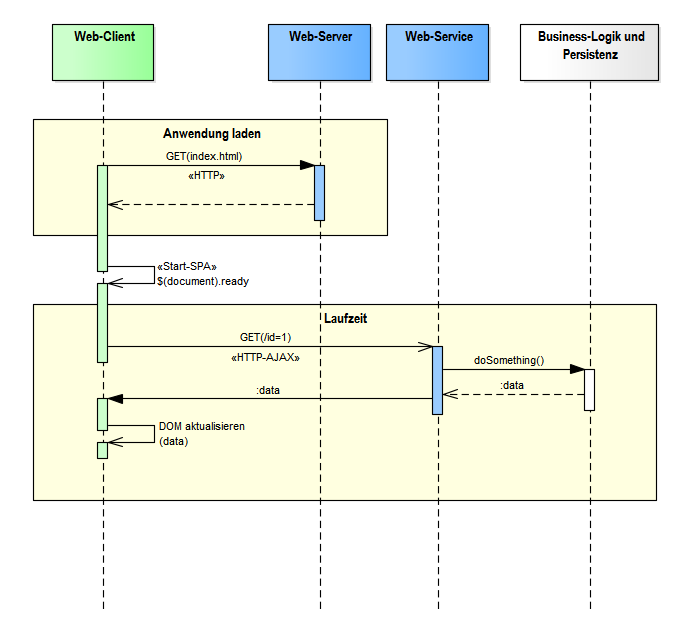
\includegraphics[width=10cm]{images/SPA_Start.png}
    \caption{Skizzierung des Ablaufs einer Single-Page-Webanwendung}
    \label{fig:spa_start}
\end{figure}

Abildung \ref{fig:spa_start} zeigt die Funktionsweise einer
Single-Page-Anwendung. Im ersten hervorgehobenen Rechteck wird das Laden der
Anwendung darstegellt. Ein Anwender ruft zum Beispiel die Webseite der
Projekt-Anwendung auf. Sein Browser schickt dann eine GET-Request nach der
\texttt{index.html}, der zentralen HTML-Seite. Diese wird vom Webserver
beantwortet. Nun hat der Anwender die Anwendung in den Speicher seines Browsers
geladen. 

Wenn nun der Anwender zum Beispiel seine Mitgliedsdaten sehen möchte, klickt er
im Browser auf den entsprechenden Link. Es wird jedoch keine neue HTML-Seite
aufgerufen und heruntergeladen, sondern die Webanwendung schickt stattdessen
eine Anfrage an einen Webservice, das \emph{Backend}. Dieser prüft dann zum
Beispiel, ob die Anfrage berechtigt ist und greift auf die Datenbank zu um die
angeforderten Daten zu lesen.

Daraufhin schickt er die Daten an die Webanwendung im Browser des Nutzers
zurück, welche dann entscheidet, wie diese Daten dargestellt werden sollen und
dann das HTML, also den Aufbau der Seite, dynamisch verändert.

Es ist also ein bisschen so, als ob der Nutzer beim Öffnen der Seite ein
Programm herunterlädt und mit diesem interagiert. Das Programm wiederum greift
auf einen Server zu, schickt und holt Daten. Schließt der Anwender das
Browserfenster löscht/deinstalliert er das Programm sozusagen.

Die Kommunikation zwischen der Anwendung im Browser und dem Webservice erfolgt
über eine Webschnittstelle. Die Anwendung ruft also Webseiten auf, wobei diese
aber nicht für Menschen gedacht sind, sondern einfach nur Daten in einer
relativ rohen Form enthalten.

\section{Die API-Spec}

Im Projekt erfolgt die Definition und Dokumentation dieser Web-Schnittstelle
über die sogenannte \href{https://wwi16ama.feste-ip.net/swagger/}{API-Spec}.
Hier werden die möglichen Routen, die die Frontend-Anwendung aufrufen kann,
definiert. Genauso werden die eventuell notwendigen Parameter der Anfragen und
die möglichen Ergebnisse beschrieben.

\begin{figure}[htpb]
    \centering
    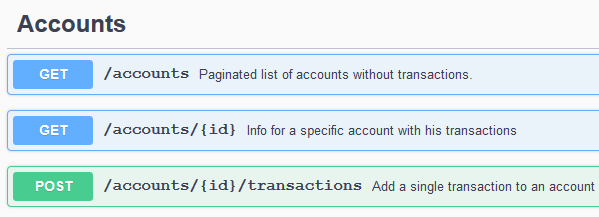
\includegraphics{images/api_spec_example_short.png}
    \caption{Übersicht der möglichen Routen zu Accounts}
    \label{fig:api_spec_accs}
\end{figure}

Abbildung \ref{fig:api_spec_accs} zeigt einen Auszug aus der API-Speck. Hier
wurden unter der Überschrift \emph{Accounts} drei verschiedene Routen
zugegriffen, auf die jeweils mit verschiedenen HTTP-Methoden zugegriffen wird.
Rechts steht eine Beschreibung, was mit dem Aufruf geschieht. Dies ist jedoch nur die Kompakt-Ansicht, die sich expandieren lässt.

Ein Ausschnitt der expandierten Darstellung ist in Abbildung
\ref{fig:api_spec_post} zu sehen. Hier wird beschrieben, welche Parameter für
die Anfrage notwendig sind. Das ist zum einen ein Parameter in der URL des
Aufrufs, um anderen muss beim \texttt{POST} eine Art Anhang mitgeschickt
werden, nämlich das Objekt im \emph{Request Body}, welches den Betrag und den
Transaktionstyp enthält.

\begin{figure}[htpb]
    \centering
    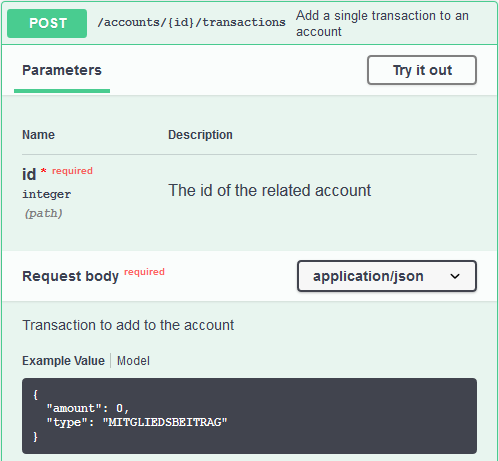
\includegraphics{images/api_spec_example_post.png}
    \caption{Notwendige Parameter für das Hinzufügen einer Transaktion zu einem
    Mitgliedskonto}
    \label{fig:api_spec_post}
\end{figure}

\section{Das Backend}

Die Umsetzung der in der API-Spec definierten Funktionalität erfolgt im
Backend. Dies ist eine Java-Applikation, welche auf einem
Tomcat-Appli\-ka\-tions\-server läuft. Die Applikation übernimmt folgende Aufgaben:

\begin{itemize}
    \item Bereitstellen der Routen
    \item Businesslogik
    \item Authentifizierung und Authorisierung
    \item Speichern in einer Datenbank
\end{itemize}

\subsection{Einstieg in Spring Boot}

Die Entwicklung erfolgt mithilfe des Frameworks
\href{https://en.wikipedia.org/wiki/Spring_Boot#Spring_Boot}{Spring Boot}. Das
Framework bietet verschiedene Features, die die Entwicklung teilweise
erleichtern. Es ist zum Beispiel möglich, einen
\href{https://de.wikipedia.org/wiki/Objektrelationale_Abbildung}{objektrelationalen Mapper}
zu nutzen, der den Datenbankzugriff start abstrahiert. Auch das Bereitstellen
des Web-Services wird durch Spring Boot vereinfacht.

Zum Einstieg in das Backend-Projekt betrachten wir die Flugzeugverwaltung. Die
findet im Paket \texttt{Plane} statt, wofür zwei Klassen und ein Interface
definiert werden (vgl. Abbildung \ref{fig:planes_package}).

\begin{figure}[htpb]
    \centering
    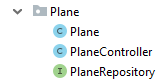
\includegraphics{images/plane_package.png}
    \caption{Inhalt des Package \texttt{Plane}}
    \label{fig:planes_package}
\end{figure}

Dabei ist die Klasse \texttt{Plane} das Business-Objekt, welches ein Flugzeug
repräsentiert. Im \texttt{PlaneController} werden die Webservice-Routen und die
Business-Logik definiert und das \texttt{PlaneRepository} abstrahiert das
Speichern von \texttt{Plane}-Objekten in der Datenbank.

Schauen wir uns nun zunächst einen Ausschnitt aus der \texttt{Plane}-Klasse an:

\begin{lstlisting}
@Entity
public class Plane {

    @Id
    @GeneratedValue(strategy = GenerationType.IDENTITY)
    private Integer id;
    private String number;
    private String name;
\end{lstlisting}

Die \lstinline{@Entity}-Annotation gibt an, dass die Klasse in der Datenbank
gespeichert werden soll, wobei die \lstinline{id} der Primärschlüssel hierfür
ist und vom Framework generiert werden soll.

\begin{figure}[htpb]
    \centering
    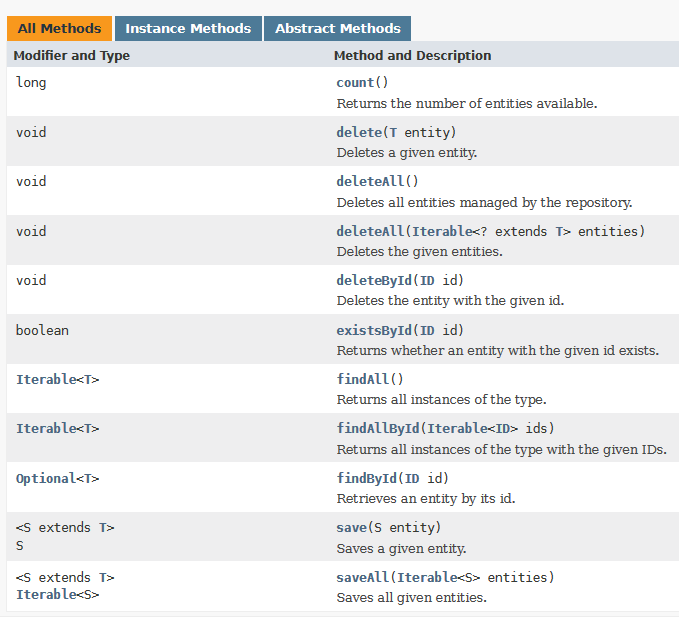
\includegraphics[width=\textwidth]{images/crudrepository.png}
    \caption{Ausschnitt der Methoden, die das PlaneRepository bereitstellt}
    \label{fig:crudrepository}
\end{figure}

Das \texttt{PlaneRepository} verwaltet dann die Datenbank-Interaktion und
stellt dafür unter anderem die Methoden aus Abbildung \ref{fig:crudrepository}
bereit. Diese Methoden erbt es von einem Interface, welches aus dem
Spring-Framework kommt. Daher wird der Datenbankzugriff in der Entwicklung
stark vereinfacht.

\begin{figure}[htpb]
    \centering
    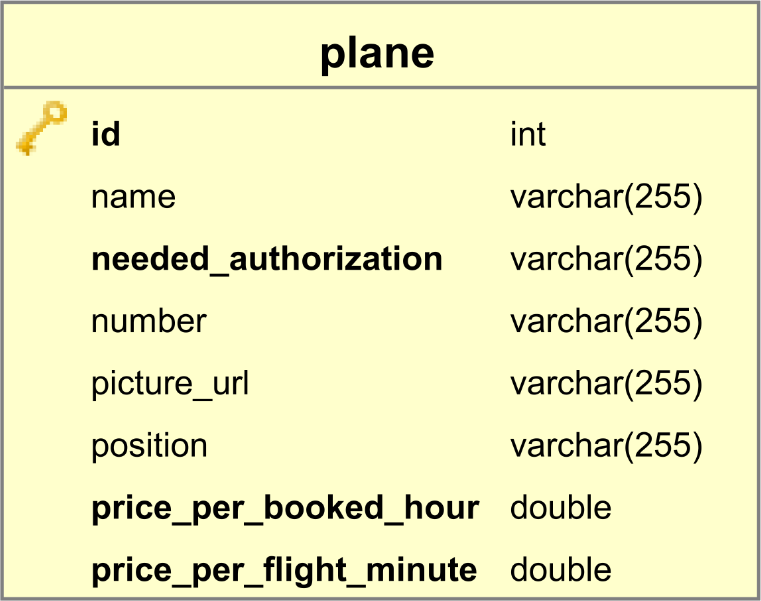
\includegraphics[width=0.4\textwidth]{images/erm/plane.png}
    \caption{Generierte Tabelle, die \texttt{Plane}-Objekte speichert}
    \label{fig:plane_table}
\end{figure}

Abbildung \ref{fig:plane_table} zeigt die MySQL-Tabelle, die vom
objekt-relationalen Mapper erstellt wurde, um die \texttt{Plane}-Objekte zu
persitieren. Diese Tabelle wird automatisch durch die Entity-Annotation
erstellt. Wenn sich die Klasse verändert, wird auch beim nächsten Start der
Applikation auch die Tabelle geändert. Durch diese Abstraktion wird ein
hypothetisches Datenbank-Team in der Entwicklung unnötig, da nur noch zu
Kontroll- und Test-Zwecken direkt auf die Datenbank zugegriffen wird.

Der \texttt{PlaneController} enthält nun die Business-Logik:

\begin{lstlisting}
@RestController
@RequestMapping(path = "planes")
public class PlaneController {
...
@GetMapping(path = "/{id}")
public Plane detail(@PathVariable int id) {

    return planeRepository.findById(id)
            .orElseThrow(() -> new NoSuchElementException();
}
...
}
\end{lstlisting}

Hier ist die Definition der unter dem Pfad \url{<server>:<port>/planes/{id}}
anzufindengen Methode gezeigt. Es wird in der URL also Parameter angegeben,
welches Flugzeug angezeigt werden soll, woraufhin das Flugzeug in der Datenbank
gesucht wird. Wird es gefunden, wird es zurückgegeben, wird kein Flugzeug
gefunden, wird eine \lstinline{Exception} geworfen. Hierbei übernimmt Spring
Boot, oder genauer, die Jackson-Bibliothek das \emph{Marshalling} und
\emph{Unmarshalling}, also das Umwandeln von JSON zu einfachen Java-Objekten
und umgekehrt. Außerdem gibt es eine Klasse, welche Exceptions fängt und
daraufhin an den Client passende Fehlermeldungen zurücksendet.

Dieser Dreiklang aus Business-Objekt, dazugehörigem Controller und Repository
ist relativ typisch für das Projekt.

\subsection{Die Business-Objekte}

Eine Übersicht über die Business-Objekte des Projekts kann das Diagramm in
Abbildung \ref{fig:erm_all} geben. Es ist dabei zu beachten, dass alle diese
Tabellen vom objekt-relationalen Mapper generiert wurden. Assoziationen werden
im Quellcode über Annotationen wie \lstinline{@OneToOne},
\lstinline{@OneToManty} und \lstinline{@ManyToMany} zwischen den Objekten
hergestellt.

\begin{figure}[htpb]
    \centering
    \includegraphics[width=\textwidth]{images/erm/all_orthogonal.png}
    \caption{Diagramm des Datenbanktabellen}
    \label{fig:erm_all}
\end{figure}

\end{document}
